\documentclass[11pt]{article}
%\usepackage{newpxtext,newpxmath}
\usepackage[left=1in,right=1in,top=1in,bottom=1in]{geometry}
\usepackage{graphicx, amsmath, amsthm, latexsym, amssymb, color,cite,enumerate, physics, framed}
\usepackage{caption,subcaption, empheq, hyperref, xcolor}
\usepackage{mathtools}
\pagenumbering{arabic}
\newtheorem{theorem}{Theorem}[section]
\newtheorem{lemma}[theorem]{Lemma}
\newtheorem{definition}[theorem]{Definition}
\newtheorem{corollary}[theorem]{Corollary}
\newtheorem{proposition}[theorem]{Proposition}
\newtheorem{convention}[theorem]{Convention}
\newtheorem{conjecture}[theorem]{Conjecture}
\newtheorem{remark}{Remark}
\newtheorem{example}{Example}
\newtheorem{solution}{Solution}
\newcommand*{\myproofname}{Proof}
\newenvironment{subproof}[1][\myproofname]{\begin{proof}[#1]\renewcommand*{\qedsymbol}{$\mathbin{/\mkern-6mu/}$}}{\end{proof}}

\newcommand{\p}{\partial}
\newcommand{\R}{\mathbb{R}}
\newcommand{\C}{\mathbb{C}}
\newcommand{\lag}{\mathcal{L}}
\newcommand{\nn}{\nonumber}
\newcommand{\ham}{\mathcal{H}}
\newcommand{\M}{\mathcal{M}}
\newcommand{\I}{\mathcal{I}}
\newcommand{\K}{\mathcal{K}}
\newcommand{\F}{\mathcal{F}}
\newcommand{\w}{\omega}
\newcommand{\lam}{\lambda}
\newcommand{\al}{\alpha}
\newcommand{\be}{\beta}
\newcommand{\x}{\xi}
\newcommand{\G}{\mathcal{G}}
\newcommand{\f}[2]{\frac{#1}{#2}}
\newcommand{\ift}{\infty}
\newcommand{\lp}{\left(}
\newcommand{\rp}{\right)}
\newcommand{\lb}{\left[}
\newcommand{\rb}{\right]}
\newcommand{\lc}{\left\{}
\newcommand{\rc}{\right\}}
\newcommand{\V}{\mathbf{V}}
\newcommand{\U}{\mathcal{U}}
\newcommand{\Id}{\mathcal{I}}
\newcommand{\D}{\mathcal{D}}
\newcommand{\Z}{\mathcal{Z}}

\hypersetup{
	colorlinks,
	linkcolor={black!50!black},
	citecolor={blue!50!black},
	urlcolor={blue!80!black}
}




\begin{document}
\begin{center}
\textbf{HYPERFINE QUANTUM BEATS \& THE MAGIC ANGLE}\\

Huan Q. Bui\\
\today
\end{center}

This document details some theory related to quantum beats, which occurs in and can affect radiative lifetime measurements. Most of the mathematical ideas are synthesized from ``\textit{Hyperfine-structure quantum beats: application of the graphical methods of angular-momentum theory to the calculation of intensity profiles}'' by Luypaert and Van Craen (1977) and Section 7.2: Quantum Beat Theory in the Density Matrix Formalism in ``\textit{Quantum Beats and Time-Resolved Fluorescence Spectroscopy}'' by S. Haroche (1976).


\begin{figure}[!htb]
	\centering
	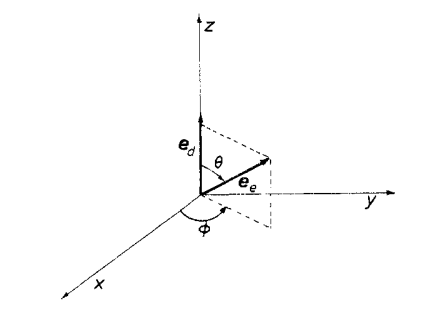
\includegraphics[scale=0.7]{beats_1}
	\caption{ Excitation-detection geometry using linear polarizers \cite{Luypaert_1977}.}
	\label{fig:scheme}
\end{figure}




\section{The Magic-Angle Problem}
Problem 9.4 of \cite{demille_atoms} on polarized fluorescence: Consider an experiment where atoms are excited with linearly polarized light, and the emitted light passes through a linear polarizer before reaching the detector. Show that if the polarization vector of the exciting light forms the ``magic angle'' $\theta_m$ given by:
\begin{equation*}
\theta_m = \arccos(1/\sqrt{3}) \approx 54.74^\circ
\end{equation*}
with the axis of the linear polarizer in front of the detector, then the detected signal is insensitive to the anisotropic part of the fluorescence. 


\begin{solution}
	blah
\end{solution}






\section{Some quantum-beat theory}

Roughly speaking, quantum beats occur due to ``interference'' in the decay of a coherent superposition of closely-spaced atomic states $\{\ket{{e}}\}$ to some collection of the final states $\{ \ket{{f}}  \}$, where $\{ \ket{{e}}   \}$ is obtained by an pulsed laser with pulse duration $\Theta \ll \tau$, the mean lifetime of $\{ \ket{{e}}   \}$. The basic scheme is given by Figure \ref{fig:energies}.

\begin{figure}[!htb]
	\centering
	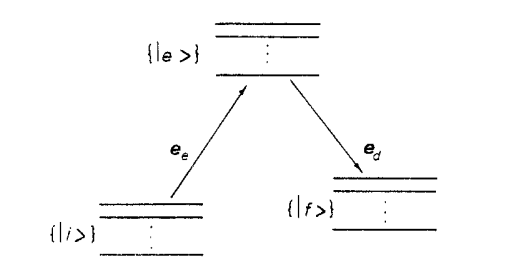
\includegraphics[scale=0.7]{energies}
	\caption{Typical quantum-beat scheme \cite{Luypaert_1977}.}
	\label{fig:energies}
\end{figure}


A short pulse of resonant light of polarization $\mathbf{e}_e$ excites an ensemble of atoms from a set of initial states $\{ \ket{i}  \}$ to $\{ \ket{e} \}$. The decay $\{ \ket{e} \} \to\{ \ket{f}  \}$ generates fluorescence light with intensity $I_{\tiny{\mbox{tot}}}(t)$. We are interested in the intensity $I(t)$ of a particular polarization $\mathbf{e}_d$ of $I_{\tiny{\mbox{tot}}}(t)$.  


In general (see Appendix \ref{app:quantum_beats}), we have
\begin{equation}\label{eq:intensity}
I(t) \propto \Tr_e\{   \rho_e(t) \mathfrak{D}  \},
\end{equation}
where $\rho_e(t)$ is the density matrix of the excited state describing the time evolution of the excited state after the pulse, and $\mathfrak{D}$ is the detection operator given in terms of the scaled-electric-dipole operator $\mathbf{D}$ as 
\begin{equation}\label{eq:detection}
\mathfrak{D} = \sum_j (\mathbf{e}_d \cdot \mathbf{D}) \ket{f}\bra{f}(\mathbf{e}_d^* \cdot \mathbf{D}).
\end{equation}
$\rho_e(t)$ is simple so long as the following conditions are satisfied:
\begin{itemize}
	\item The excitation is broadline, i.e., the spectral width of the exciting light is much bigger than the inverse of the duration of the pulse. 
	\item The excitation is weakly-coupled to the atomic system, i.e., the duration of the pulse is much less than the average time between two successive photon absorptions by an atom. 
	\item The duration of the pulse is shorter than the mean lifetime $\tau$ of $\{ \ket{e} \}$, and is less than the inverse Bohr frequencies $\omega_{e,e'}$ corresponding to the excited-state energy differences. 
\end{itemize}
Under these conditions \textcolor{blue}{(which I believe our experiment satisfies)}, the density matrix $\rho_e(t)$ has the following property:
\begin{equation}\label{eq:density}
\bra{e} \rho_e(t) \ket{e'} = \sum_{ii'} \bra{e} \mathbf{e}_e \cdot \mathbf{D} \ket{i} \bra{i} \rho_i(-T) \ket{i'} \bra{i'} \mathbf{e}_e^* \cdot \mathbf{D} \ket{e'} \exp\lb -(i\omega_{ee'} + \Gamma_e) t \rb,
\end{equation}
where $\rho_i(-T)$ is the density matrix of the initial state. Here, $\Gamma_e = \tau_e^{-1}$. Putting Eq. \ref{eq:density} into Eq. \ref{eq:intensity} and Eq. \ref{eq:detection} we find
\begin{align}
I(t) \propto \sum_{f,ii',ee'} &\bra{e} \mathbf{e}_e \cdot \mathbf{D} \ket{i} \bra{i} \rho_i(-T) \ket{i'} \bra{i'} \mathbf{e}_e^* \cdot \mathbf{D} \ket{e'} \nonumber \\
&\times \bra{e'}\mathbf{e}_d \cdot \mathbf{D} \ket{f}\bra{f}\mathbf{e}_d^* \cdot \mathbf{D} \ket{e} \exp\lb -(i\omega_{ee'} + \Gamma_e) t \rb.
\end{align}






\section{Hyperfine-structure quantum beats}




\section{Example: Linearly-polarized excitation and detection}



\section{Spatial Anisotropy of the Emitted Radiation}



\appendix

\section{Quantum Beat Theory in the Density Matrix Formalism \cite{haroche}}\label{app:quantum_beats}

\textcolor{blue}{fill in the background for the ``quantum beat theory'' section here...}




\bibliographystyle{unsrt}
\bibliography{quantum_beats}
\end{document}